\documentclass [12pt,twoside]{article}
\usepackage[utf8]{inputenc}
\usepackage[T1]{fontenc}

%Page margins, header and footer positions
\usepackage{geometry}
\geometry{
    a4paper,
    total={210mm,297mm},
    left=25mm,
    right=25mm,
    top=30mm,
    bottom=25mm,
    headsep=7mm}

\interfootnotelinepenalty=10000

%To display filling dots in the TOC for all entries
\usepackage[titles]{tocloft}
\renewcommand{\cftsecleader}{\cftdotfill{\cftdotsep}}

%Define new header and footer style
\usepackage{fancyhdr}

\pagestyle{fancy}
\fancyhf{}
\lhead{\color{Gray}{\small{CLup project by Davide Luca Merli, Dario Passarello}}}
\lfoot{\textcolor{Gray}{\small{Copyright © 2020, Davide Luca Merli, Dario Passarello – All rights reserved}}}
\rfoot{\textcolor{Gray}{\thepage}}
\renewcommand{\headrulewidth}{0pt}

%PACKAGES
\usepackage{wasysym}
\usepackage{pifont}

\newcommand{\supported}{\ding{52}\xspace}
\newcommand{\unsupported}{\ding{55}\xspace}
\newcommand{\partsupported}{\textcolor{black!40}{\ding{52}}\xspace}
\newcommand{\lowsupported}{\textcolor{black!20}{\ding{52}}\xspace}
\newcommand{\unknowsupported}{\textbf{?}\xspace}

%Font: Times
% \usepackage{times}
%Change monospaced font
\renewcommand{\ttdefault}{lmtt}

%tables
\usepackage{tabu}
\usepackage{tabularx}
\usepackage{ltablex}
\usepackage{longtable}
\usepackage{float} % To allow the use of H modifier in long tables

%landscape mode
\usepackage{pdflscape}
\usepackage{rotating}
\usepackage{caption}

%make landscape mode be sensitive to even and odd pages
%start
\def\myrotate{\ifodd\c@page\else-\fi 90}
\makeatletter
\global\let\orig@begin@landscape=\landscape%
\global\let\orig@end@landscape=\endlandscape%
\gdef\@true{1}
\gdef\@false{0}
\gdef\landscape{%
    \global\let\within@landscape=\@true%
    \orig@begin@landscape%
}%
\gdef\endlandscape{%
    \orig@end@landscape%
    \global\let\within@landscape=\@false%
}%
\@ifpackageloaded{pdflscape}{%
    \gdef\pdf@landscape@rotate{\PLS@Rotate}%
}{
    \gdef\pdf@landscape@rotate#1{}%
}
\let\latex@outputpage\@outputpage
\def\@outputpage{
    \ifx\within@landscape\@true%
        \if@twoside%
            \ifodd\c@page%
                \gdef\LS@rot{\setbox\@outputbox\vbox{%
                        \pdf@landscape@rotate{-90}%
                        \hbox{\rotatebox{90}{\hbox{\rotatebox{180}{\box\@outputbox}}}}}%
                }%
            \else%
                \gdef\LS@rot{\setbox\@outputbox\vbox{%
                        \pdf@landscape@rotate{+90}%
                        \hbox{\rotatebox{90}{\hbox{\rotatebox{0}{\box\@outputbox}}}}}%
                }%
            \fi%
        \else%
            \gdef\LS@rot{\setbox\@outputbox\vbox{%
                    \pdf@landscape@rotate{+90}%
                    \hbox{\rotatebox{90}{\hbox{\rotatebox{0}{\box\@outputbox}}}}}%
            }%
        \fi%
    \fi%
    \latex@outputpage%
}
\makeatother
%end

%graphics
\usepackage{graphicx}
\usepackage[dvipsnames, table]{xcolor}
%If you upload images from PC, you need to insert code for the path here (different for Windows and Unix OS)

%References
%\usepackage{xpatch}
%\usepackage[backend=biber, style=numeric, citestyle=numeric, sorting=none]{biblatex}
%\addbibresource{main.bib}

%Other
\usepackage{ifthen}
\usepackage{xspace}
\usepackage{enumitem}
\usepackage{amssymb}
\usepackage[pdftex, colorlinks]{hyperref}
\newcommand{\comment}[1]{{\color{Red}$\blacktriangleright$ Comment: #1 $\blacktriangleleft$}}


% Some utilities\ldots
\usepackage{soul}
\usepackage{tikz}

\usetikzlibrary{calc}
\usetikzlibrary{decorations.pathmorphing}


\makeatletter

\newcommand{\defhighlighter}[3][]{%
  \tikzset{every highlighter/.style={color=#2, fill opacity=#3, #1}}%
}

\defhighlighter{yellow}{.5}

\newcommand{\highlight@DoHighlight}{
  \fill [ decoration = {random steps, amplitude=1pt, segment length=15pt}
        , outer sep = -15pt, inner sep = 0pt, decorate
       , every highlighter, this highlighter ]
        ($(begin highlight)+(0,8pt)$) rectangle ($(end highlight)+(0,-3pt)$) ;
}

\newcommand{\highlight@BeginHighlight}{
  \coordinate (begin highlight) at (0,0) ;
}

\newcommand{\highlight@EndHighlight}{
  \coordinate (end highlight) at (0,0) ;
}

\newdimen\highlight@previous
\newdimen\highlight@current

\DeclareRobustCommand*\highlight[1][]{%
  \tikzset{this highlighter/.style={#1}}%
  \SOUL@setup
  %
  \def\SOUL@preamble{%
    \begin{tikzpicture}[overlay, remember picture]
      \highlight@BeginHighlight
      \highlight@EndHighlight
    \end{tikzpicture}%
  }%
  %
  \def\SOUL@postamble{%
    \begin{tikzpicture}[overlay, remember picture]
      \highlight@EndHighlight
      \highlight@DoHighlight
    \end{tikzpicture}%
  }%
  %
  \def\SOUL@everyhyphen{%
    \discretionary{%
      \SOUL@setkern\SOUL@hyphkern
      \SOUL@sethyphenchar
      \tikz[overlay, remember picture] \highlight@EndHighlight ;%
    }{%
    }{%
      \SOUL@setkern\SOUL@charkern
    }%
  }%
  %
  \def\SOUL@everyexhyphen##1{%
    \SOUL@setkern\SOUL@hyphkern
    \hbox{##1}%
    \discretionary{%
      \tikz[overlay, remember picture] \highlight@EndHighlight ;%
    }{%
    }{%
      \SOUL@setkern\SOUL@charkern
    }%
  }%
  %
  \def\SOUL@everysyllable{%
    \begin{tikzpicture}[overlay, remember picture]
      \path let \p0 = (begin highlight), \p1 = (0,0) in \pgfextra
        \global\highlight@previous=\y0
        \global\highlight@current =\y1
      \endpgfextra (0,0) ;
      \ifdim\highlight@current < \highlight@previous
        \highlight@DoHighlight
        \highlight@BeginHighlight
      \fi
    \end{tikzpicture}%
    \the\SOUL@syllable
    \tikz[overlay, remember picture] \highlight@EndHighlight ;%
  }%
  \SOUL@
}

\makeatother

% Common abbrev. are set as commands to ensure proper spacing after the dot
\RequirePackage{xspace}
\newcommand{\ie}{i.e.\@\xspace}
\newcommand{\aka}{a.k.a.\@\xspace}
\newcommand{\Ie}{I.e.\@\xspace}
\newcommand{\cf}{cf.\@\xspace}
\newcommand{\Cf}{Cf.\@\xspace}
\newcommand{\eg}{e.g.\@\xspace}
\newcommand{\Eg}{E.g.\@\xspace}
\newcommand{\etal}{et al.\@\xspace}
\newcommand{\etc}{etc.\@\xspace}
\newcommand{\wrt}{w.r.t.\@\xspace}
\newcommand{\Wrt}{W.r.t.\@\xspace}



\date{}

\begin{document}
%TITLE PAGE

\begin{titlepage}
  \begin{center}

    \HUGE \textbf{CLup} \\[0.5cm]
    \LARGE Customers Line-Up \\[0.5cm]
    \hspace*{-1.2cm}
\includegraphics[scale=0.5]{../../logo/clup_logo_nobg.png}

    \vfill

    \Huge \textbf{Implementation Document} \\
    \LARGE Implementation Document \\[2cm]

    \begin{multicols}{2}
      \large
      \begin{flushleft}
        Software Engineering II Project \\
        Computer Science and Engineering\\
        Politecnico di Milano\\
        Version 1.0 - 10 January 2021 \\
      \end{flushleft}
      \begin{flushright}
        
\includegraphics[scale=0.6]{Images/PolimiLogo.png} \\
        Davide Merli - 10578363\\
        Dario Passarello - 10566467 \\
      \end{flushright}
    \end{multicols}
  \end{center}

\end{titlepage}

%Define deliverable specific info
%Replace cell contents where needed
\begin{table}[h!]
  \begin{tabu} to \textwidth { X[0.4,r,p] X[0.7,l,p] }
    \hline

    \textbf{Deliverable:}   & Implementation Document                                                \\
    \textbf{Title:}         & Implementation Document                                                \\
    \textbf{Authors:}       & Davide Merli, Dario Passarello                                         \\
    \textbf{Version:}       & 1.0                                                                    \\
    \textbf{Date:}          &    07 February 2021                                                    \\
    \textbf{Download page:} & https://github.com/davidemerli/MerliPassarello/                        \\
    \textbf{Copyright:}     & Copyright © 2020, Davide Merli, Dario Passarello – All rights reserved \\
    \hline
  \end{tabu}
\end{table}




\setcounter{page}{2}


%------------------------------------------------------------------------------------------------------------------------------------------------
\newpage
\addcontentsline{toc}{section}{Table of Contents}
\tableofcontents
\newpage
\addcontentsline{toc}{section}{List of Figures}
\listoffigures
\addcontentsline{toc}{section}{List of Tables}
\listoftables

%------------------------------------------------------------------------------------------------------------------------------------------------
\clearpage
\section{Introduction}
\label{sect:introduction}
\subsection{Purpose}
The purpose of this document is to analyze and describe deeply the design choices of the software and the system to be, which is described in the CLup Requirements Analysis and Specifications Document (RASD).

Design decisions will be further explained together with the architectural structure of the system as a whole as well as its subsystems.

\medskip

This document will also provide insights about Implementation and Testing, by outlining the characteristics of CLup subsystems and interfaces. Every component will be analyzed and put into perspective with the others, in order to deploy a plan for the developement, the organization and the parallelization of the work.

\subsection{Scope}

Due to the recent coronavirus global pandemic, many of the human activities have been drastically affected and restricted by the need to contain the virus diffusion. Norms and regulations may vary from contry to country, but almost everywhere the main focus is to mantain social distancing to avoid diffusion from one person to another.
One of the most difficult activity to fullfil (yet absolutely essential) is grocery shopping.
\medskip

Stores are forced to restrain access to avoid too many people inside the building, and this produces endless lines out of the stores. This can both increase the danger for people waiting for their turn and force the shops to regulate customers even outside the structure.

\medskip

CLup aims to reduce heavily the issues involving customer queues outside of stores by permitting clients to keep track of their position in the store queue or book in a visit in advance with an easy to use application.

\clearpage
\subsection{Definitions, Acronyms, Abbreviations}

\subsubsection{Acronyms}

\begin{itemize}
    \item \textbf{S2B}: Software To Be
    \item \textbf{RASD}: Requirement Analysis and Specifications Documents
    \item \textbf{REST}: REpresentational State Transfer
    \item \textbf{API}: Application Programming Interface
    \item \textbf{UX}: User Experience
    \item \textbf{UI}: User Interface
    \item \textbf{SSO}: Single sign-on
    \item \textbf{QR code}: Quick Response code
    \item \textbf{OS}: Operating System
    \item \textbf{RAM}: Random Access Memory
    \item \textbf{LAN}: Local Area Network
    \item \textbf{GPS}: Global Positioning System
    \item \textbf{GB}: GigaByte
    \item \textbf{TCP/IP}: Transmission Control Protocol/Internet Protocol
    \item \textbf{HTTPS}: Hypertext Transfer Protocol Secure
    \item \textbf{IoT}: Internet of Things
    \item \textbf{MQTT}: Message Queuing Telemetry Transport
    \item \textbf{RAID}: Redundant Array of Independent Disks
    \item \textbf{UML}: Unified Modeling Language
    \item \textbf{TDD}: Test-driven development
\end{itemize}

\vfill
\pagebreak

\subsubsection{Definitions}

\begin{itemize}
    \item \textbf{Access controller}: a subsystem that permits the entrance of customers into the store. It can be a device like a smart turnstile that reads customers tickets or just a person of the store staff manually scanning tickets.
    \item \textbf{Business account}: a CLup account that is destined to store managers or operators and therefore the 'business' side of CLup
    \item \textbf{In-Site ticket}: a ticket that is taken by a customer near the store. It can be both a virtual paperless ti an emitter near the store premises
    \item \textbf{Virtual ticket}: a ticket issued through the CLup application
    \item \textbf{Physical/Paper ticket}: a printed physical ticket, emitted by a printer near the store premises
    \item \textbf{Valid Ticket} (at time X): a ticket that has a code recognized by the CLup system and valid for the specified time
    \item \textbf{Time slot}: a time delta that is associated with a number of bookable tickets (which varies and is customizable from store to store)
    \item \textbf{People-Counting System}: a subsystem that permits the counting of the number of people inside the store. It can comprehend a device like a proximity sensor or a smart turnstile, or it can be a person of the store staff manually counting people.
    \item \textbf{Customer Application}: the CLup mobile application destined to customers that want to shop inside stores adopting CLup
    \item \textbf{Operator Application}: the CLup mobile application destined to store staff to monitor entrances and statistics
    \item \textbf{Store Main System}: the store main server that communicates directly with CLup servers. All store subsystems and smart devices should communicate with it through an Intranet
    \item \textbf{Geocoding API}: Geocoding converts addresses into geographic coordinates to be placed on a map. A Geocoding API allows the use of their services to permit translation between textual addresses and Latitude/Longitude coordinates
    \item \textbf{Map API}: An external services that provides operations of geographics maps and the download of map information, usually of the places in proximity of given geographics coordinates
    \item \textbf{Hashed Password}: When a password has been “hashed” it means it has been turned into a scrambled representation of itself. A user's password is taken and – using a key known to the site – the hash value is derived from the combination of both the password and the key, using a set algorithm.
    \item \textbf{Time to market}: is the length of time it takes from a product being conceived until its being available for sale.
    \item \textbf{Alpha Test}: a trial of machinery, software, or other products carried out by a developer before a product is made available for beta testing.
    \item \textbf{Beta Test}: a trial of machinery, software or other products in the final stages of development, carried out by a party unconnected with the development process.
    \item \textbf{DevOps}: is a set of practices that combines software development (Dev) and IT operations (Ops). It aims to shorten the systems development life cycle and provide continuous delivery with high software quality.
    \item \textbf{Quality Assessment}: is the data collection and analysis through which the degree of conformity to predetermined standards and criteria are exemplified.
\end{itemize}

\subsection{Revision History}

\begin{itemize}
    \item 1.0: 10 January 2021 - First Release
\end{itemize}

\subsection{Reference Documents}

\begin{itemize}
    \item R\&DD Assignment A.Y. 2020-2021 - Elisabetta di Nitto, Matteo Giovanni Rossi
    \item Software Engineering II slides and material - Elisabetta di Nitto, Matteo Giovanni Rossi
    \item CLup RASD - Davide Luca Merli, Dario Passarello
    \item \href{https://material.io/design}{Material Design Guidelines}
    \item \href{https://www.conventionalcommits.org/en/v1.0.0/}{Convetional Commits Guidelines}
    \item \href{https://git-scm.com/}{Git - versioning system}
\end{itemize}

\subsection{Used Tools}
\begin{itemize}
    \item Umlet - for UML diagrams
    \item Draw.io - for other diagrams
    \item Proto.io - for UI Mockups
    \item Github - for code hosting and version control
    \item \LaTeX \space  - to write this entire document
    \item Visual Studio Code + Latex Workshop - as a \LaTeX \space environment
\end{itemize}

\clearpage

\subsection{Document Structure}

\textbf{Chapter 1} explains the purpose of this document, summarizes the scope of the CLup project and the relation between this Design Document and the Requirement Analysis and Specifications Document.
Acronyms and Definitions used through the whole document are listed and explained.
It provides the history of the document revisions and this very description of all the chapters, together with the documents used as a reference.

\medskip

\textbf{Chapter 2} presents the system on various levels of detail. An high level view is provided to further frame CLup as a system composed of different software running on different platforms and devices. Component Diagrams illustrate all the components of the various subsystems. Every component is defined and described, exhibiting its role in the system and how it communicates with other internal or external components.

\medskip

\textbf{Chapter 3} shows the most meaningful interfaces of the CLup Application, giving a nice idea of what the final product will look like from a customer's perspective.

\medskip


\textbf{Chapter 4} associates every component described in section \ref{sect:architectural_design} with the Requirements they contribute to satisfy, as a direct reference for developers.

\medskip


\textbf{Chapter 5} is another direct reference for developers as it expresses how the developement process will be organized, how and in which order the components of the whole system are to constructed. The same is done with the testing: how it relates to the developement process, how component are tested, and which technologies are to be employed.

\medskip

\textbf{Chapter 6} shows the time spent from each member of the team for writing this document.

%------------------------------------------------------------------------------------------------------------------------------------------------
\clearpage
\section{Requirements and Functionalities Implemented}
\label{sect:requirements_functions}
The prototype functionalities focus on the 'line-up' feature, the customer could only retrieve a ticket to enter the store as soon as there is space. The 'book a visit' feature is not implemented.
The scope of the prototype is showing how the system works from the point of view of the customer. For this reason the prototype focuses on the User Experience. The management side is kept at a bare minimum providing only the store operator functions to call customer to the entrance, scan tickets and view real time data about the store crowdedness. The system does not provide functions to insert new stores, neither to create new operator account, but some random data is provided to the testers in order to be able to test the system.
\subsection{Component and Deployment View}
With respect to the Design Document, to ease and speedup the task of developing a prototype some components were moved or removed.
\begin{figure}[h!t]
    \centering
    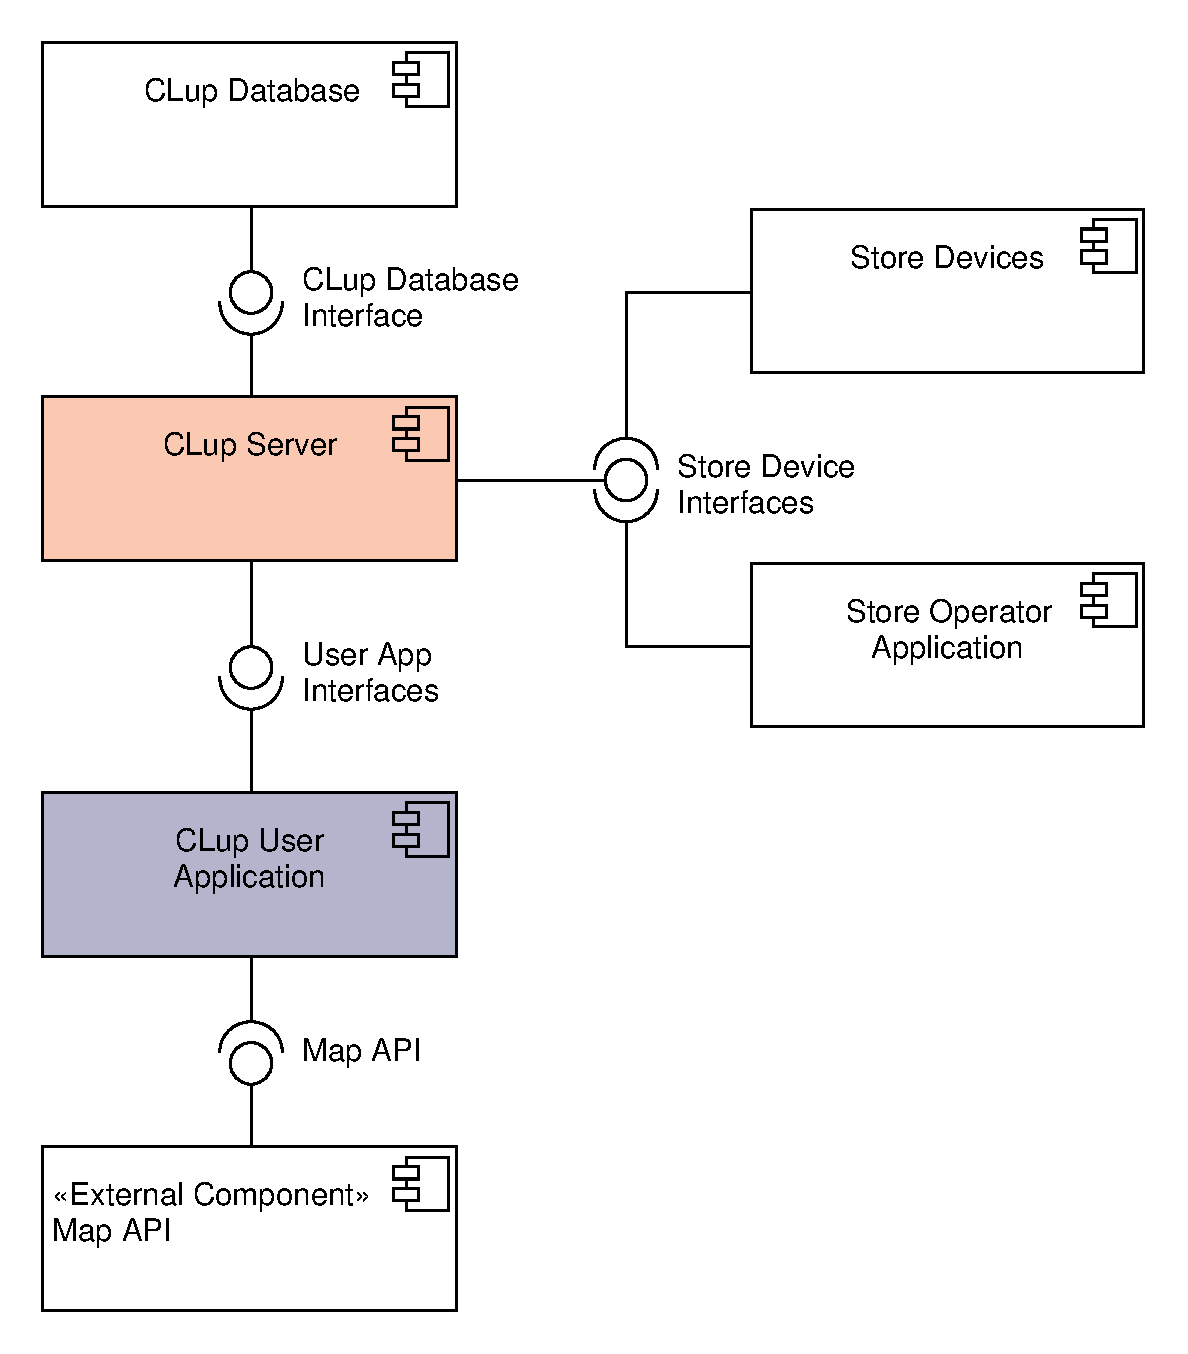
\includegraphics[width=\textwidth]{Images/UML_general_component.pdf}
    \caption{\label{fig:General Component}Implemented Component Diagram}
\end{figure}

\pagebreak

In the DD the original component diagram moved the functions handled from the store out to the CLup server. This is convenient when the two systems handle different types of tickets and different type of statistics to collect but in the case of the prototype there is only one type of ticket to handle. In the prototype is useless to split the two macro components so they are merged in a unique backend macro-component called CLup Server in the diagrams. 
\begin{figure}[h!t]
    \centering
    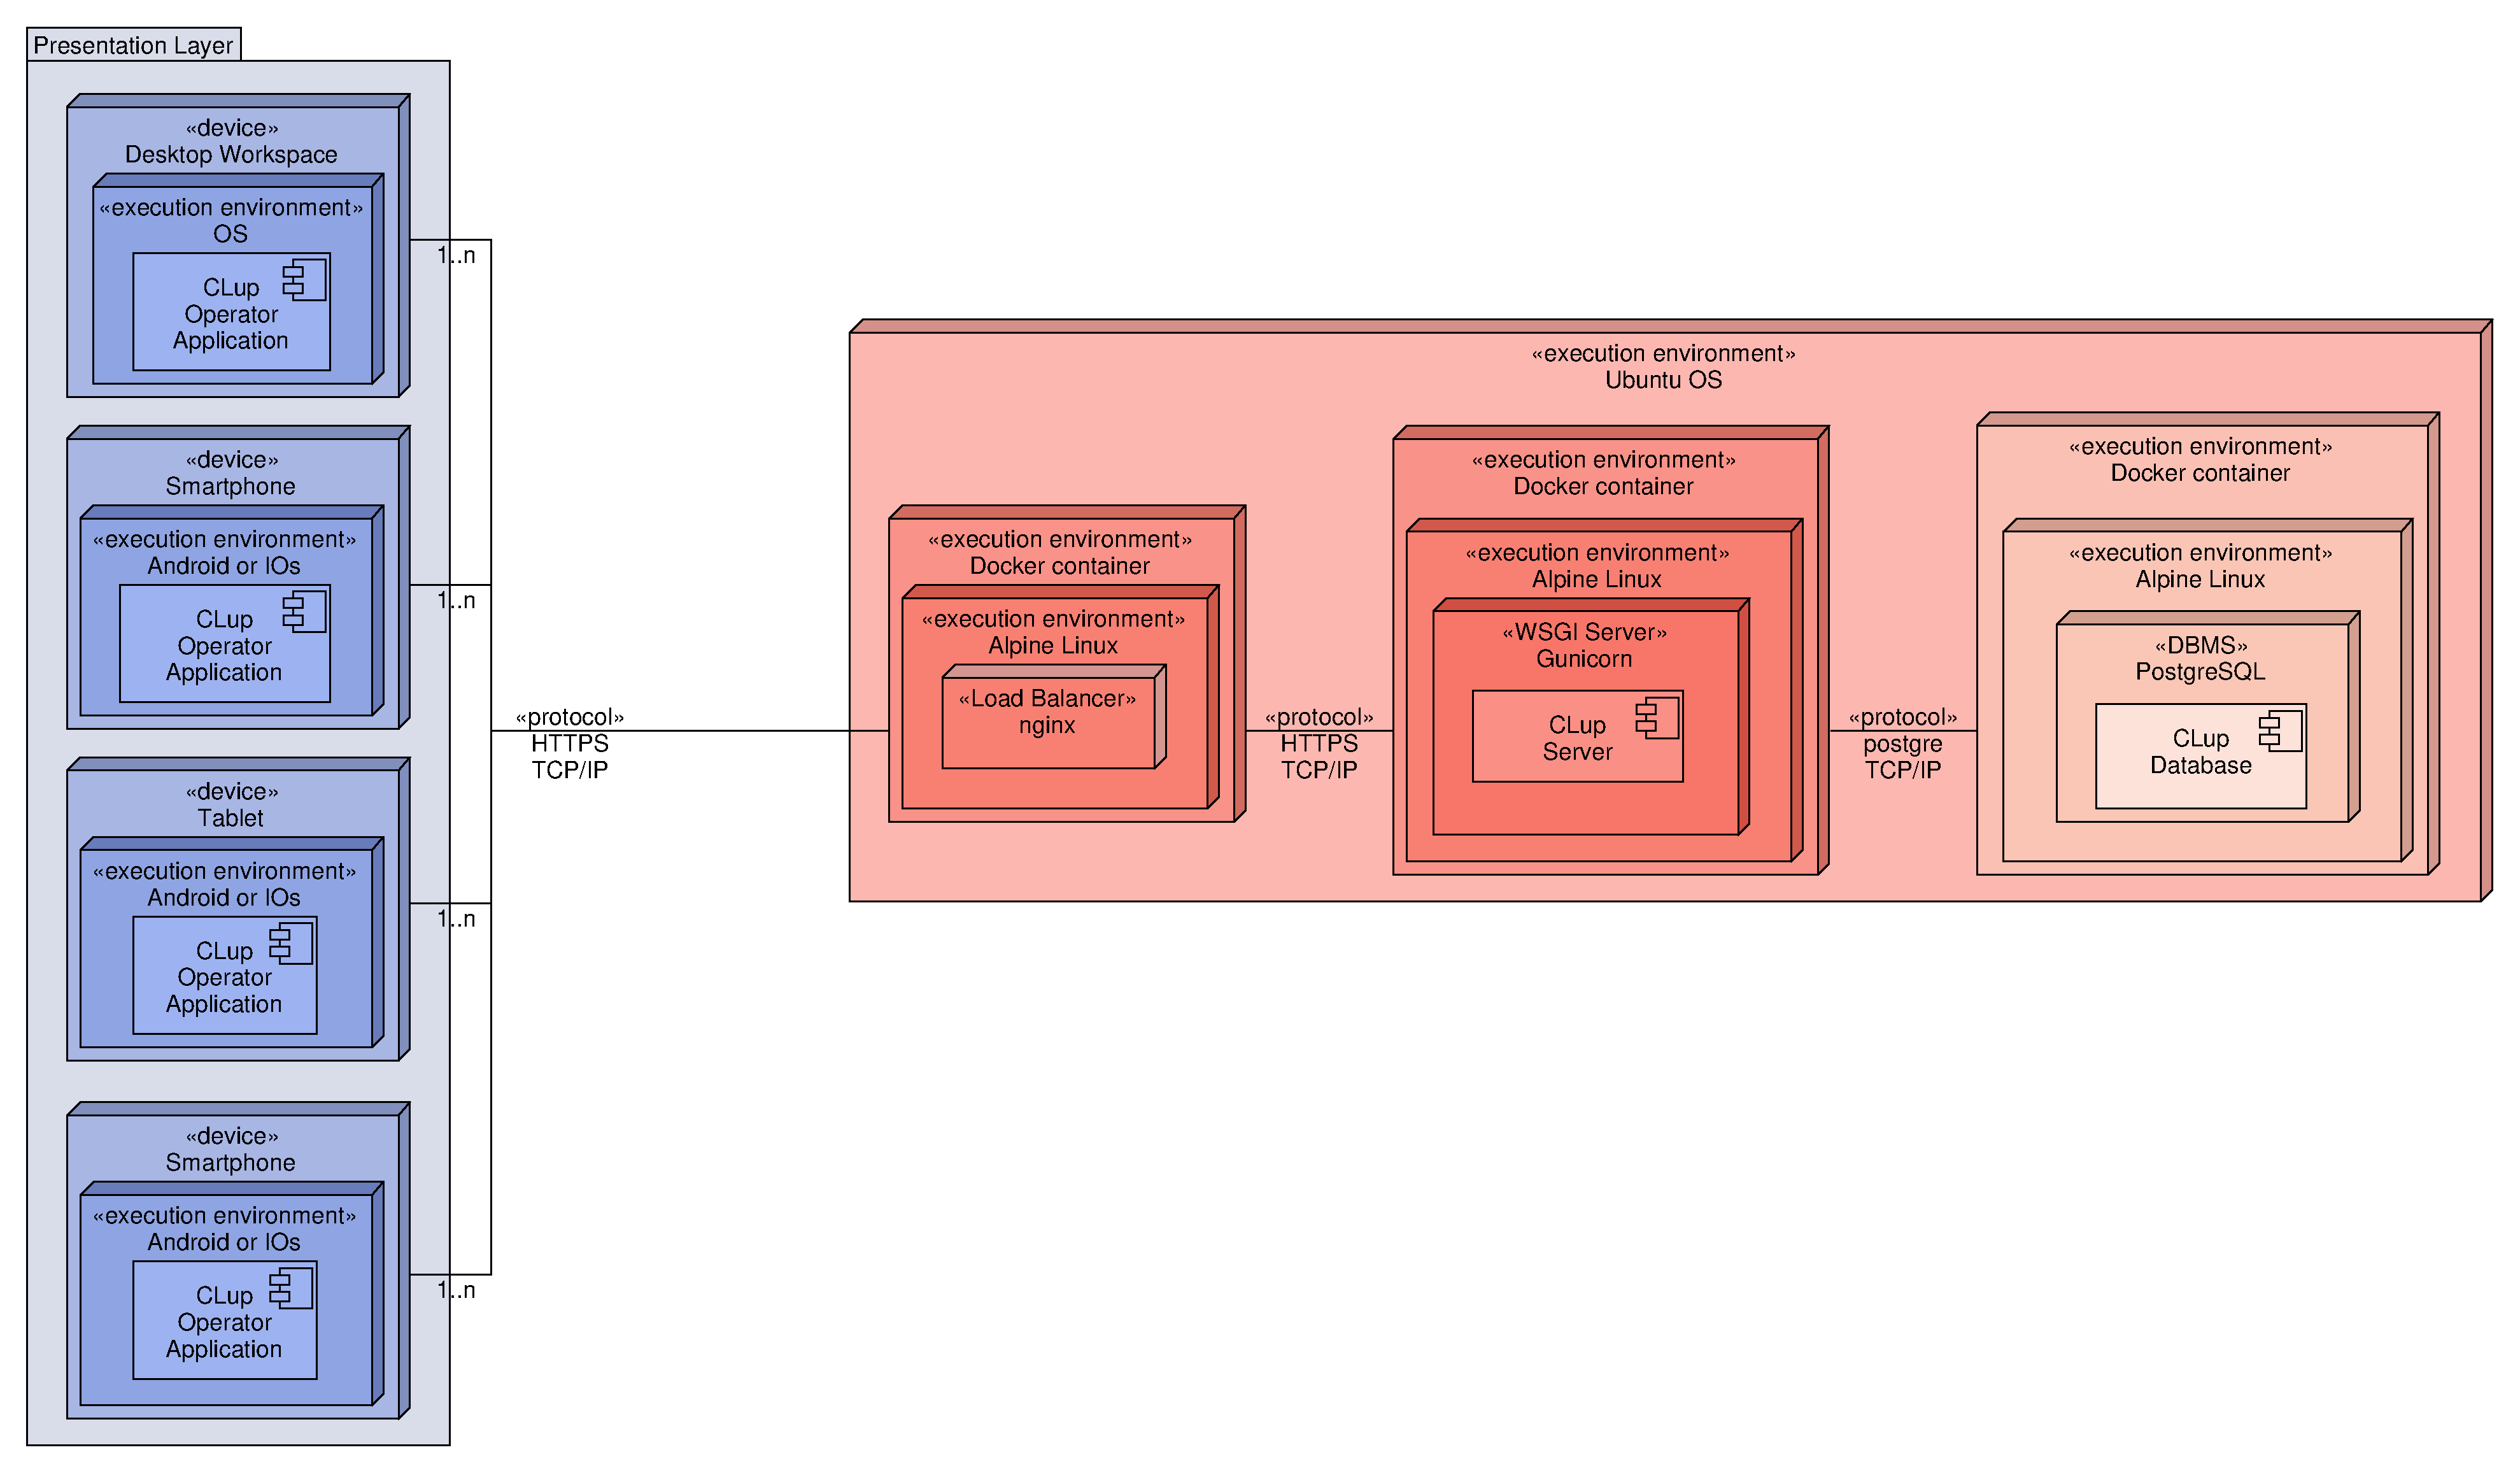
\includegraphics[width=\textwidth]{Images/UML_deployment_diagram.pdf}
    \caption{\label{fig:General Component}Prototype Deployment Diagram}
\end{figure}

Due to the merger of the two components the backend now could run in a single machine isolating the different modules in containers. 



\rowcolors{2}{gray!25}{white}
\renewcommand{\arraystretch}{1.4}
\captionof{table}{Requirements table}
\begin{tabular}{C{1cm}L{11cm}C{3.1cm}}
    \rowcolor{gray!50}
    Label & Requirement description & Implemented?                                                                                                                                                                     \\

    R1   & The system must keep general information and contacts about the store chains adopting CLup & No                                                                                                 \\
    R2   & The system must provide each store a store-admin account  & No                                                                                                                              \\
    R3   & The store-admin account must allow the creation of store-operator accounts &               No                                                                                                   \\
    R4   & For each store the system must allow the users to retrieve information about location and business hours   & Partially                                                                                \\
    R5   & The system stores information about capacity of each market & Yes                                                                                                                                \\
    R6   & The system won't let anyone enter the store if the maximum capacity has been reached  & Yes                                                                                                      \\
    R7   & The system will let a customer enter the store if and only if they have a a valid ticket  & Yes                                                                                                     \\
    R8   & The system will use the occupancy data retrieved from the store to control the store access      & Yes                                                                                    \\
    R9   & The system must provide an interface to communicate with the store access control     & Yes                                                                                                   \\
    R10   & The system must provide an interface for user to compile a shopping list  & No                                                                                                                  \\
    R11   & The system must take in consideration shopping list data and historic data from previous user visits to reduce store crowdedness per department & No                                            \\
    R12   & The system must allow the store-admin account to create and edit entrance time intervals & No                                                                                                   \\
    R13   & Each time interval must have a number of bookable slots fewer than the store capacity & No                                                                                                      \\
    R14   & The system must allow authenticated users to book a visit in a desired time interval & No                                                                                                        \\
    R15   & The system must not allow a user to book a slot in an already full time interval     & No                                                                                                       \\
    R16   & The system must not allow a user to book a visit if he has already reserved another visit  & Yes                                                                                                 \\
    R17   & The system must allow a customer to create a numbered virtual queue ticket and notify them if he can enter immediately (if the store is not full) or provide them a waiting time estimation & Partially\\
    R18   & The system must notify the customers with a virtual queue ticket when it's time to approach the store entrance  & Partially                                                                            \\
    R19   & The store operator application must allow an authenticated operator to manually admit customers & No                                                                                            \\
\end{tabular}

\vfill

\begin{tabular}{C{1cm}L{11cm}C{3.1cm}}
    \rowcolor{gray!50}
    Label & Requirement description & Implemented?                                                                                                                                                          \\
    R20   & The system  must ask the customer to provide the estimated visit time when booking a time slot   & No                                                                               \\
    R21   & The system must allow stores to hand out numbered physical queueing tickets to those that do not use the CLup application & Partially                                                       \\
    R22   & The system must allow the access to the store to customer with numbered tickets using a 'First Come First Served' logic, treating virtual and physical ticket owner equally  & Yes   \\
    R23   & The system must try to estimate waiting time based on store capacity, reservations and the current number of people with numbered tickets waiting in line  & No                      \\
    R24   & The system should interface with an screen placed at the entrance of the store to notify customer which ticket numbers will enter in the next called batch  & Partially                    \\
    R25   & The system must let the store-admin accounts retrieve statistics collected from CLup regarding their store & No                                                                      \\
    R26   & The system must record periodically and store statistics about the occupancy of each store & Yes                                                                                     \\
    R27   & The customer CLup application must show brief statistics about average occupancy of each stores during different days of the week  & No                                             \\
    R28   & The operator CLup application must show to an authenticated operator the real time occupancy of the store & Yes                                                                      \\
    R29   & The customer CLup application must be cross-platform and must work on the majority of the devices & Yes                                                                               \\
    R30   & The stores adopting CLup must be displayed on a map & Yes                                                                                                                            \\
    R31   & The CLup customer application allows user to mark stores as favorite in order to access them quickly                                                                            \\
    R32   & The CLup customer app after the login allows immediately to book tickets right from the homepage & Yes                                                                               \\
    R33   & The system must provide an interface for automated control devices to communicate to CLup data about store entrances, store leavings and crowdedness in the various departments & Partially\\
    R34   & The system must push notifications to user devices with update information on the store he has a ticket for   & Partially                                                                  \\
    R35  & The system must associates tickets with line numbers & Yes                                                                                                                           \\
    R36  & The system allows customer to register an user account & Yes \\
    R37  & The system allows registered customers to authenticated & Yes\\
\end{tabular}
\vfill
\subsection{Partially Implemented Features}
\begin{itemize}
    \item \textbf{R4 For each store the system must allow the users to retrieve information about location and business hour}: The store location feature is implemented (in order to display stores in the map). The business hours are not provided to the user, this feature could be implemented using an external API with opening times or storing these opening times in the database
    \item \textbf{R17 The system must allow a customer to create a numbered virtual queue ticket and notify them if he can enter immediately (if the store is not full) or provide them awaiting time estimation}: The waiting time estimation is not provided. To estimate the waiting time an accurate model based on historical data could be used.
    \item \textbf{R18 The system must notify the customers with a virtual queue ticket when it’s time to approach the store entrance}:
    The push notification component is not implemented in the prototype so the server can't push message to the user application. However the client will check if the ticket has been called by pulling data from the server API periodically.
    \item \textbf{R21 The system must allow stores to hand out numbered physical queueing tickets to those that do not use the CLup application}:
    The CLup server provides an API for this feature but for satisfying this requirement a ticket printer is required. 
    \item \textbf{R25 The system should interface with an screen placed at the entrance of the store to notify customer which ticket numbers will enter in the next called batch}:
    Similar to R21
    \item \textbf{R33 The system must provide an interface for automated control devices to communicate to CLup data about store entrances, store leavings and crowdedness in the various departments}: Similar to R21. The departments' crowdedness control feature is not implemented in the prototype



\end{itemize}



%------------------------------------------------------------------------------------------------------------------------------------------------
\clearpage
\section{Adopted Frameworks}
\label{sect:adopted_frameworks}
The implementation of the CLup prototype is divided in two parts: Frontend and Backend. 

\subsection{Backend Frameworks and Languages}

\subsubsection{CLup Server and API}
The framework chosen for the backend is Flask. Flask is a lightweight WSGI web application framework written in python. Flask is very good for prototyping web application and APIs because it very easy to set up (it could be installed in one command from the python package installer PIP) and comes with a debug mode that speeds up the debugging process.
Along with flask some other libraries are used to build the CLup Server Api.
\begin{itemize}
    \item \textbf{SQLAlchemy} is a Object Relational Mapper library (ORM). An ORM allows to map the database entities and the relationship between them to objects and references in the application code. The ORM will translate operations on the objects to SQL queries that will be executed to the database. The ORM decouples the application from the database. In this way the application code is independent from which underlying DBMS, and the latter could be changed without changing the application code.
    \item \textbf{Marshmallow} is a marshalling library for python, well integrated with flask. Marshalling consists in converting objects from the memory in a format ready for storage or transmission. Marshmallow makes the validation the request inputs a lot simpler so the programmer doesn't need to write a lot of error-prone boilerplate code for the input validation
    \item \textbf{Flask-RESTful} The CLupServer API uses the RESTful architectural style. Flask-RESTful simplifies the code writing of this API providing to the programmer a software interface to declare each endpoint as a class, containing the different HTTP methods accepted from the endpoints. For example to implement an endpoint that allows to create ticket with a POST request is sufficient to declare a class `CreateTicket' that extends the class Resource (provided from FlaskRestful), and implement the post() method.
    \item \textbf{Flask-Jwt-Extended} is a library for handling the authentication in flask using JWT tokens. A JWT token is an encoded string generated from the server and given to the user after checking its credentials. The JWT contains the user e-mail, an expiration timestamp and an hash for checking integrity. The JWT token is generated when the user does login request. Every request done by the user must contain this token so, flask-jwt-extended will check the validity of the token at each request. With flask-jwt-extended, allowing the access to an API endpoint to only the authenticated user is very straightforward, it's enough to put a python annotation before the endpoint methods for which authentication is needed.
\end{itemize}
\subsubsection{Data layer}
Regarding the data model a SQL relational database is preferred to a noSQL one, because the data to persist has a well defined Entity-Relation structure (i.e. Tickets, Users, Store\ldots).

For the Data layer a postgreSQL DBMS is adopted. PostgreSQL is a production ready open-source relational SQL database. It's stable and used in a lot of commercial applications so it's a good fit for the CLup prototype.

\subsubsection{Development Tools}
Different development tools are used when writing and debugging the backend code.
\begin{itemize}
    \item \textbf{Poetry} is a tool that helps managing the dependencies of a project, setting them up in an isolated python environment. Isolating the execution environment is essential to enhance the portability and the maintainability of the software. When poetry is set up it will create automatically a virtual python environment for the project and resolve the dependencies.
    \item \textbf{Black} is an automatic python code formatter. Black formats the code according to the PEP-8 standard, enhancing the readability.
    \item \textbf{pytest} is the official python testing framework. (More about the testing on section 5)
\end{itemize} 

\subsubsection{Deployment Tools}
\textbf{Docker} is an useful tool to automatically build and ship applications. A Docker application is made of different containers each one running a different application, these application could communicate using an internal network.

For this prototype docker is employed to build and deploy the backend using a single command. 
Without docker each component (i.e. CLup Server Application, Database, Load Balancer) should be set up manually.

\medskip

For deploying the application in production it is not recommended the use of the flask development WSGI server. So the CLup Server Application container runs a \textbf{gunicorn} server.

\medskip

\textbf{Nginx} is a broadly used load balancer. Due to the low usage of a prototype application, a load balancer is not strictly needed, but it is included for enhancing the stability of the gunicorn server and could be useful for having better performance when stress testing the system.

\subsection{Frontend}
\subsubsection{Flutter}

For the application frontend we decided to use the Flutter framework considering its many advantages:
\begin{itemize}
    \item Flutter allows to natively compile applications for every major platform, including Android, IOs, Web and Desktop applications. By using a single code base it is possible to deliver the same experience to every platform, and without the need to define different teams for every version.
    \item Natively compiling applications ensures good performances even if not writing native code for the specific target platforms.
    \item Flutter provides lots of predefined Widgets\footnote{Every component in a Flutter application is a Widget, and every displayed page is a Tree of Widgets, one inside the other; working with Widgets allows to only rebuild the parts of the application that need to be updated, which improves performance.} for every kind of situation. This allows for faster developement since every common behavior in a classic application is already usable out of the box
    \item There are lots of libraries (both official and third party libraries) that further populate the list of usable Widgets (i.e. libraries to draw graphs with statistics, map integration, HTTP requests, QR code scanning/generation)
    \item Flutter allows for 'Hot Reloading', which instantly rebuilds the application while debugging, and without necessarly restarting the application, speeding up the developement processruns onruns on
    \item Flutter is written with the Dart programming language, which is very flexible, has very powerful features (like Mixins and Extensions Methods, but also a very polished null safety implementation) and resembles Java in the general syntax (which is a known language to team members)
    \item Team members already had some experience with the framework
\end{itemize}

On the other hand, Flutter has some downsides:
\begin{itemize}
    \item Flutter Web is still in beta developement, so it has not been tested enough to be considered 'stable', but the developement of the framework is very active, and behind the project there is Google.
    \item Some low level features, for example the interaction with background tasks in the various operating systems running the application, are not yet supported natively (in Dart code) but may require small amounts of codes to be written in the respective native languages (i.e. Java/Kotlin for Android, Swift for IOs)
\end{itemize}


%------------------------------------------------------------------------------------------------------------------------------------------------
\clearpage
\section{Requirement Traceability}
\label{sect:source_structure}
\subsection{Backend Source Structure}
All the backend code is stored in the ITD/CLupServer folder.
\begin{lstlisting}
    CLupServer\

    |-- docker-compose.yml
    |-- docker-compose-testing.yml
    |-- build.sh
    |-- test.sh
    |-- clup-server\
    |-- data\
    |-- db_config\
\end{lstlisting}

\begin{itemize}
    \item \textbf{docker-compose.yml}: docker-compose configuration file for setting up the production server. Docker-compose will read this file and build/set-up the containers accordingly.
    \item \textbf{docker-compose-testing.yml}: docker-compose configuration file for running the tests. Docker-compose will read this file and build/set-up the containers accordingly, containerizing all components but not the flask server.
    \item \textbf{build.sh}: A shell script that builds (if not already done) and starts the docker containers of the production server.
    \item \textbf{test.sh}: A shell script that starts the docker containers and runs pytest.
    \item \textbf{data}: Contains nginx configuration files.
    \item \textbf{db-config} Contains a SQL script that runs when the PostgreSQL is created. This script creates the databases (clup, clup-testing)
\end{itemize}

\begin{lstlisting}
    CLupServer\clup-server\

    |-- CLup.py
    |-- wsgi.py
    |-- config.py
    |-- data.json
    |-- docker-entrypoint.sh
    |-- Dockerfile
    |-- poetry.lock
    |-- pyproject.toml
    |-- README.rst
    |-- requirements.txt
    |-- clup_server\
    |-- tests\


\end{lstlisting}

\begin{itemize}
    \item \textbf{CLup.py}: The startup script for the flask application. This script is used to run the project when flask is not containerized. Some optional flag could be passed to this script (preceded by two dashes):
          \begin{itemize}
              \item dev:  For setting up Flask in development mode
              \item drop: For dropping the database content on startup
              \item populate: For populating the CLupUser and Store tables from the sample data stored in data.json
          \end{itemize}
    \item \textbf{wsgi.py}: The startup script for the application when it is run from a production WSGI server (i.e. Gunicorn). This is startup script is used when the app is containerized.
    \item \textbf{config.py}: Stores the configuration variables for flask for Development mode and for Production mode. The JWT secret key for the Production server is taken from the environment variables to avoid publishing the secret in the repository. The secret should be set to a random string (using export) before starting the server (This is automatically done from the build.sh script).
    \item \textbf{data.json}: Contains fake Stores and Users data to populate the database.
    \item \textbf{docker-entrypoint.sh}: A shellscript executed from Docker when it starts the application container. This script starts gunicorn.
    \item \textbf{Dockerfile}: Contains the instructions to allow Docker to build the application container.
    \item \textbf{pyproject.toml}: Configuration file for poetry. Contains the list of all the library dependencies needed to run the project.
    \item \textbf{requirements.txt}: Configuration file for pip. Used from the application container to retrieve all the project dependencies.
    \item \textbf{clup-server}: Contains the application python package
    \item \textbf{tests}: Contains the integration tests
\end{itemize}

\begin{lstlisting}
    CLupServer\clup-server\

    |-- __init__.py
    |-- models.py
    |-- schemas.py
    |-- routes.py
    |-- orm.py
    |-- auth_manager.py
    |-- information_provider.py
    |-- queue_manager.py
    |-- ticket_manager.py

\end{lstlisting}

\begin{itemize}
    \item \textbf{\_\_init\_\_.py} is the package initialization file, executed by Python when the clup-server package is imported from another source file. Here is implemented the application factory method createApp(). This method allows multiple instances with different configurations to be created. The createApp methods will import all the other modules in the package and then starts to inizialize all the needed resources. For example it will start the database connection, configure the API routes\ldots
    \item \textbf{models.py} contains all the models class declarations. Each model class is mapped to a database table, and SQLAlchemy provides the translation to a SQL statement for every operation made on a instance of one of the model classes. Each class contains also methods to decouple the data layer management code from the business code executed at each API call
    \item \textbf{routes.py} registers on start up all the API routes exposed to be accessed by the application
    \item \textbf{auth-manager.py} contains the APIs and the business logic for authenticating customers and operators.
    \item \textbf{information-provider.py} contains the APIs that provide information about the stores.
    \item \textbf{queue-manager.py} contains the APIs and the business logic used by the store operators(or automated control systems) to get the status of the queue and manage it
    \item \textbf{ticket-manager.py} contains the APIs to create, view and cancel tickets.
\end{itemize}


\subsection{Frontend Source Structure}

All the frontend code is stored in the ITD/clup\_application folder.

\begin{lstlisting}
    clup_application\

    |-- android\
    |-- assets\
    |-- fonts\
    |-- ios\
    |-- lib\
    |-- test\
    |-- web\
    |-- .gitignore
    |-- .metadata
    |-- pubspec.lock
    |-- pubspec.yaml
    |-- README.md 

\end{lstlisting}

\begin{itemize}
    \item \textbf{android/}: folder containing mostly configuration files to correctly build the android application. Most of these are autogenerated files, with little tweaks, for example to setup Android permissions.
    \item \textbf{assets/}: here are stored all the needed assets files (in this case only the CLup logo).
    \item \textbf{fonts/}: contains the collection of fonts used in the application.
    \item \textbf{ios/}: configurations to build the IOs application. has not been tweaked since the team had hardware limitations and could not test IOs builds.
    \item \textbf{lib/}: contains the whole Flutter code of the application.
    \item \textbf{web/}: contains configuration files for the webapp build.
    \item \textbf{.gitignore}: autogenerated by Flutter, avoids pushing build and other local configuration files to the git repo
    \item \textbf{.metadata}: file used by Flutter to track the properties of the Flutter project. Autogenerated and should not be manually edited.
    \item \textbf{pubspec.lock}: autogenerated, used by Flutter to store information about dependencies
    \item \textbf{pubspec.yaml}: main configuration file for the dependencies of the Flutter project.
    \item \textbf{README.md}: text to be displayed in the git repo to provide info about the folder.
\end{itemize}



\begin{lstlisting}
    lib\

    |-- api\
    |------- authentication.dart
    |------- information_provider.dart
    |------- operator_utils.dart
    |------- ticket_handler.dart
    |-- conditional_deps\
    |------- key_finder_stub.dart
    |------- keyfinder_interface.dart
    |------- mobile_keyfinder.dart
    |------- web_keyfinder.dart
    |-- gps\
    |------- gps_component.dart
    |-- pages\
    |------- login_page.dart
    |------- map_page.dart
    |------- operator_page.dart
    |------- signup_confirm_page.dart
    |------- signup_page.dart
    |------- store_view_page.dart
    |------- ticket_page.dart
    |-- configs.dart
    |-- generated_plugin_registrant.dart
    |-- main.dart

\end{lstlisting}

\begin{itemize}
    \item \textbf{api/}: this package contains all the calls to the CLup API tranformed in simple utils as in a Facade pattern, for easy access throughout the whole application.
    \item \textbf{conditional\_deps/}: this packages contains different implementations of local storage management, to avoid a problem when working with crossplatform applications in Flutter; it is not possible to ship an application with web libraries as dependencies, so the application instantiates different behaviours to correctly match the underling environment.
    \item \textbf{gps/}: in this packages is present the code that is used to retrieve the user location. The method determinePosition() controls them location permissions to use the gps sensor, and in case of no sensor or no permissions, makes a call to an external API to geolocalize using the ip address.
    \item \textbf{pages/}: this package contains all the pages of the application, and the majority of the code takes care of the layouts, the visual componenents, and the buttons. There is very little application logic, since all the work is done on the backend.
    \item \textbf{configs.dart}: contains global variables like URLS and custom colors, to be easily accessed throughout the whole application.
    \item \textbf{generated\_plugin\_registrant.dart}: autogenerated by google\_maps\_flutter\_web, not to be edited manually.
    \item \textbf{main.dart}: code to create and launch the application, here is defined the theme of the CLup app, the hierarchy structure of the pages, and utils function to write/read from local storage (implementing the correct keyfinder from the conditional dependencies).
\end{itemize}

%------------------------------------------------------------------------------------------------------------------------------------------------
\clearpage
\section{Testing}
\label{sect:testing}
\subsection{Backend}
The testing in the backend is performed using pytest.
Pytest is the official testing framework for python.
The testing metodology adopted for the backend is the AAAC pattern.
AAAC stands for Arrange Act Assert Cleanup.
\begin{itemize}
    \item \textbf{Arrange}: In this phase the resource needed for the test (fixtures) are created. For example the connection with the database is created, the test data are loaded, the mocks are instantiated.
    \item \textbf{Act}: The function to test is executed and its results are collected
    \item \textbf{Assert}: The results collected from the previous phase are compared with the expected results. If there is something different than what was expected an Assertion Error is raised, and the test fails.
    \item \textbf{Cleanup}: After the test has been executed the resourced are dropped, side effects from the tests are restored (i.e. rollback database transactions).
\end{itemize}

\subsubsection{Fixtures}
A \textbf{fixture} is a resource that is needed for setting up the test (Arrange phase).

Example of fixtures are a file with test inputs, a connection with an API or a database\ldots

Pytest allows to give a different scope to each fixture. A fixture could last for the entire test session, or could be used only for a single test or for a group of tests.

Here is an example of a pytest fixture
\begin{lstlisting}[language=python]
    #Scope could be function, class, module...
    @pytest.fixture(scope=session)
    def a_fixture(fixture_dependency_1, fixture_dependency_2,...):
        #Arrange fixture
        ... 
        yield fixture 
        #Cleanup fixture
\end{lstlisting}
As shown a fixture could depend from other fixture. For example in the CLup prototype the database connection depends on the start of the flask application, and the test data to write in the database depends from the database connection.


\subsubsection{Flask testing}
Flask is really easy to test. A flask application in development mode offers a test client that could simulate the request sending to the client. In this prototype this client is used as fixture to test all the different API endpoints.

\subsubsection{Unit tests}
Unit tests aren't really useful for a simple application like this. Writing a unit test required to write a stub for the database component that is already tested by the postgreSQL team! This requires too much effort compared to the benefits, so it turned to be not so useful. Instead integration tests with the CLup Server component and the CLup database are performed for this implementation.

\subsubsection{Integration Tests}
The integration test is performed using the test client provided by flask and aims to test the integration between the CLup Server and the database. There are different small tests for the edge cases  for most of the APIs and a bigger test that simulated the complex evolution of the queue in a supermarket, performing all the possible operations in the queue. The test were performed in local on a test database different from the production database using test data stored in `data.json'.

\subsubsection{Statement Coverage}
The statement coverage is calculated using pytest-cov, a plugin for pytest. The coverage of the statement is about 85\%, that is an acceptable value considering that there are a some statements that are not accessible because they are executed only during the first setup of the system.
\begin{figure}[h!t]
    \centering
    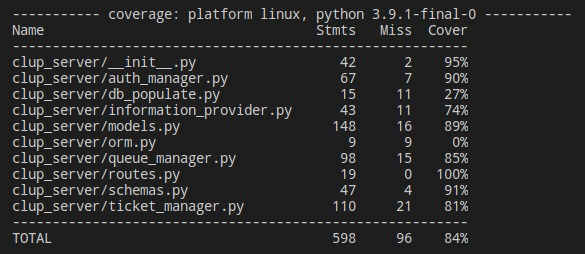
\includegraphics[width=\textwidth]{Images/coverage.jpeg}
    \caption{\label{fig:General Component}Statement Coverage}
\end{figure}

%------------------------------------------------------------------------------------------------------------------------------------------------
\clearpage
\section{Installation}
\label{sect:installing}
\subsection{Backend}
The backend server has been deployed with Docker containers on AWS.



\subsubsection{Starting the server}
An instance of the server has already been deployed online using AWS, and the API is available at https://clup.waifocus.com so it's not needed to run it locally.
If you want it is still possible to run the server locally on Linux or on Windows Subsystem of Linux (WSL)

\textbf{Installation steps}
\begin{enumerate}
    \item Install \href{https://docs.docker.com/get-docker/}{Docker}
    \item Install \href{https://docs.docker.com/compose/install/}{Docker Compose}
    \item Check if Docker service is running. If not start it with the command
          \begin{lstlisting}[language=bash]
    sudo systemctl start docker
    \end{lstlisting}
    \item  Open build.sh and change the JWT\_SECRET\_KEY string to another value. When running the application in a production environment keep this value secret.
    \item Run the script with
          \begin{lstlisting}[language=bash]
    ./build.sh
    \end{lstlisting}
          this script will create the containers by invoking docker-compose. If you didn't add your user in the docker group
          you have to run the script with sudo
    \item You can do requests the address localhost:8000
\end{enumerate}

\clearpage

\subsubsection{Running tests}
For running pytest a startup script that doesn't containerize the application is available.
\textbf{Installation steps}
\begin{enumerate}
    \item Install \href{https://docs.docker.com/get-docker/}{Docker}
    \item Install \href{https://docs.docker.com/compose/install/}{Docker Compose}
    \item Check if Docker service is running. If not start it with the command
          \begin{lstlisting}[language=bash]
    sudo systemctl start docker
    \end{lstlisting}
    \item Install \href{https://python-poetry.org/}{Poetry}
    \item Open a linux shell and go in CLupServer/clup-server
    \item Run the command
          \begin{lstlisting}[language=bash]
    poetry install
    \end{lstlisting}
    \item Run the test script with
          \begin{lstlisting}[language=bash]
    ./test.sh
    \end{lstlisting}
          The script sets up all the containers and the flask application in testing mode and the it runs the Pytest.
          If you didn't add your user in the docker group
          you have to run the script with sudo
    \item (Optional) If you want to start the application out of the container run the command
          \begin{lstlisting}[language=bash]
    poetry run python3 CLup.py  - -dev  - -populate
    \end{lstlisting}
\end{enumerate}

\subsection{Frontend}

\subsubsection{Flutter Mobile Application}
The application has been developed and tested only on Android, due to limitation in the available hardware.

To install the application we provide two~.apk packages:
\begin{itemize}
    \item RELEASE Version: A smaller package containing the prototype as it would be released in a production environment, downloadable here
    \item DEBUG Version: A bigger package containing the debug version of the prototype, which is useful for checking potential error messages, full content of API calls, etc. Downloadable here
\end{itemize}

\subsubsection{Flutter Web Application}
A release version of the web application has been deployed using Github Pages, and it is available at https://clup-mp.github.io, without the need to install anything.

We also provide a package containing all files to deploy the web application, downloadable here

To test locally the web application it is possible to setup a simple web server, for example by using python:
\begin{lstlisting}[language=bash]
    python3 -m http.server
\end{lstlisting}
Then opening a browser on http://localhost:8000



%------------------------------------------------------------------------------------------------------------------------------------------------
\clearpage
\section{Effort Spent}
\label{sect:effort}
\subsection{Dario Passarello}
\begin{itemize}
    \item Meetings on how interface backend with frontend: 4 hrs
    \item Backend project setup: 4 hrs
    \item Learning new skills in backend development: 8 hrs
    \item Coding backend: 22 hrs
    \item Writing backend tests: 7 hrs
    \item Deploying backend: 6 hrs
    \item Final system test: 3 hrs
    \item Writing ITD documentation: 8 hrs
\end{itemize}
Total: 62 hours

\subsection{Davide Luca Merli}
\begin{itemize}
    \item Meetings on how interface backend with frontend: 4 hrs
    \item Frontend project setup: 1h
    \item Documenting on Flutter features, best practices, external libraries: 8h
    \item Frontend development: 40h
    \item Deploying WebApp: 2 hrs
    \item Final system test: 4 hrs
    \item Writing ITD documentation: 6 hrs
\end{itemize}
Total: 65 hours


% %------------------------------------------------------------------------------------------------------------------------------------------------
% \clearpage
% \addcontentsline{toc}{section}{References}
% \bibliographystyle{plain}
% \bibliography{main}
% %------------------------------------------------------------------------------------------------------------------------------------------------



\end{document}
